% -*- mode: LaTeX; coding: utf-8; -*-

\chapter{Web-palvelut}

Web-palveluilla tarkoitetaan järjestelmiä, jotka kommunikoivat
keskenään käyttäen vakiintuneita Web-tekniikoita. Web-palvelimet eivät
ole riippuvaisia mistään tietystä laitteisto- tai
käyttöjärjestelmäarkkitehtuurista. Web-palveluiden käyttämät
teknologiat eivät sinänsä ole erityisen vallankumouksellisia, mutta
tiedonvaihdon helpottuminen standardien protokollien ja Web:n
hajautetun rakenteen ansiosta on tehnyt Web-palveluista
mielenkiintoisia niin kehittäjien kuin käyttäjienkin
näkökulmasta\cite{javaweb}.

IBM määrittelee Web-palvelut seuraavasti: ``Web-palvelut ovat
itsenäisiä ja modulaarisia sovelluksia, jotka voidaan julkistaa,
määritellä, paikallistaa ja suorittaa verkon ylitse, yleeensä WWW:n
välityksellä.''\cite[s.4]{websecurity}

Tietoturvan kannalta WWW-palvelut ovat haastavia, koska niitä
käytetään Internetin välityksellä eivätkä ne ole rajoittuneita
esimerkiksi tietyn organisaation lähiverkkoon. Myös osia
WWW-palveluista sijaitsee usein fyysisesti eri paikoissa ja ne
kommunikoivat keskenään Internetin välityksellä.

Tässa luvussa käsitellään komponentteja, joista tämänhetkiset
Web-palvelut koostuvat. Erityistä huomiota on kiinnitetty seikkoihin,
jotka vaikuttavat palvelun tietoturvaan.

\section{Palvelinohjelmistot}

Web-palveluiden toteuttajan näkökulmasta lähin komponentti on
palvelinohjelmisto. Se käsittelee HTTP-kyselyt ja lähettää vastauksina
käyttäjän selaimessa näytettäviä ja prosessoitavia osia, kuten
hypertekstiä, kuvia ja komentosarjoja.

Web-palvelinohjelmisto ei välttämättä kommunikoi suoraan palvelun
käyttäjän tietokoneen kanssa vaan välissä käytetään usein välimuistipalvelua,
joka vähentää palvelimelle kohdistuvaa rasistusta säilyttämällä
harvoin muuttuvaa sisältöä välimuistissa ja välittämällä tätä suoraan
käyttäjille. Muuttuva tai välimuistille uusi sisältö pyydetään
palvelinohjelmistolta.

Internet-tietoturvapalveluita tarjoavan Netcraftin raportista
huhtikuulta 2010~\cite{netcraft} käy ilmi, että kaksi suurinta
Web-palvelinalustaa ovat \textit{Apache} (53.93~\% suosituimmista
sivuista), \textit{Microsoft} (24.97~\%). Näiden jälkeen tulevat
\textit{Google} ja \textit{nginx} kumpikin 6~\% osuudella.

Tuloksia voi vääristää jonkin verran se, että joissakin tapauksissa
edustalla suoritetaan välimuistipalveluna toista palvelinohjelmistoa,
esimerkiksi Apachea tai nginx:ä, joka välittää kyselyt eteenpäin
varsinaiselle Web-palvelinohjelmistolle. Tämä selittää esimerkiksi
sen, miksi Zope puuttuu kokonaan suosituimpien palvelinten
joukosta. Esimerkiksi Jyväskylän yliopiston Web-palvelimena näkyy
tilastoinnissa Apache, vaikka Web-palvelu on toteutettu
Zope-palvelinohjelmiston päällä suoritettavalla Plonella. Samoin on
käynyt Tomcat-palvelimella ajettavalle Korppi-o\-pin\-to\-tie\-to\-jär\-jes\-tel\-mäl\-le.

\subsection{Apache}

Suosituimpana palvelinalustana Apache on luonnollisesti suosittu kohde
myös tietomurtojen yrityksille. Apachesta itsestään on kuitenkin
löydetty verrattain vähän
tietoturva-aukkoja. Suurin osa tietomurroista
keskittyykin murtamaan varsinaista Web-palvelua palvelinalustan
sijaan.  % tämä on oletus, FIXME etsi lähde tai poista

Apache pystyy suorittamaan komentosarjoja perinteisen CGI-rajapinnan
lisäksi myös palvelinlaajennosten avulla, jolloin saavutetaan
tiiviimpi integraatio ja enemmän suorituskykyä verrattuna
CGI-rajapintaan~\cite{cginopeus}.

Apachea voidaan suorittaa lukuisissa eri käyttöjärjestelmissä,
mukaanlukien Linux ja Windows. Suosittuja Apache-alustalla
käytettäviä ohjelmointikieliä ovat PHP ja Python. Tunnettuja tässä
ympäristössä käytettäviä Web-palveluita ovat mm. Wikipediassa
käytettävä MediaWiki ja lukuisilla selainkäyttöisillä
keskustelupalstoilla käytettävä phpBB. Ympäristöä, jossa on käytössä
Linux, Apache, MySQL ja PHP, kutsutaan usein nimellä LAMP.

\subsection{IIS}

Apachen jälkeen toiseksi suurinta markkinaosuutta web-palvelinalustoista pitää Microsoftin kehittämä Internet Information Services (lyh. IIS). Ensimmäisen versio sovelluksesta
julkaistiin NT-käyttöjärjestelmälle vuona 1996, ja vuonna 2008 julkaistiin IIS 7 Windows Server 2008 palvelinjakelun yhteydessä. Uusin virallinen versio sovelluksesta on tällä hetkellä   
IIS 7.5, ja siitä on ladattavissa 180-päivän ilmainen kokeiluversio Windows Server 2008 alustalle Microsoftin sivuilta \cite{IIS}.

Aikaisemmista IIS-versioista on löydetty paljon eri tasoisia tietoturvariskejä, joista tunnetuin on Code Red Wormiksi nimetty hyökkäys, joka saastutti yli kolmesataatuhatta web-sivustoa.
Hyökkäys pohjautui puskuriylivuotoon, johon Microsoft oli julkaissut päivityksen kuukausi takaperin, mutta jota osa palveluita ylläpitävistä tahoista ei ollut asentanut. Tämän hyökkäyksen
johdosta yleinen käsitys IIS-sovellusten tietoturvasta on vähintäänkin kyseenalainen. Uusimmista versioista ei ole kuitenkaan löydetty vastaavanlaisia tietoturvariskejä, ja Secunian
ylläpitämän listan mukaan uusimmasta versiosta ei löydy yhtään paikkaamatonta tietoturvariskiä \cite{Secunia}.

Suurin muutos uusimmissa versioissa verrattaessa vanhoihin on siirtyminen modulaariseen arkkitehtuuriin. Tämä mahdollistaa uusien komponenttien nopean lisäämisen ja poistamisen, jonka lisäksi  
monipuolinen API-rajapinta tarjoaa mahdollisuuden tehdä yksilöllisiä komponentteja omiin tarpeisiin. Modulaarinen rakenne parantaa myös sovelluksen tietoturvaa pienentämällä asennettavien 
osien määrää ainoastaan niihin, joita ylläpitäjä tarvitsee. Tietoturvaan ja skaalautuvuuteen on muutenkin kiinnitetty enemmän huomiota alusta asti, joiden lisäksi monet Apachen ominaisuuksista
kuten URL-osoitteiden uudelleenkirjoitus on otettu käyttöön \cite{IIS}. IIS:n suurimpana haittapuolena nykyisin sen onkin sidonnaisuus Windows-maailmaan, sillä muille alustoille sitä ei ole 
saatavilla. Tästä huolimatta IIS on nykyisin varteenotettava vaihtoehto Apachelle tietynlaisessa ympäristössä. 

\subsection{Zope}

Vaikka Apachen ja Microsoft IIS:n markkinaosuudet kattavat suurimman osan käytetyistä web-alustoista, on markkinoilla suuri määrä pienempiä ratkaisuja, joille löytyy oma käyttäjäkuntansa. Yksi 
näistä on vapaaseen lähdekoodiin pohjautuva Zope \cite{Zope}. Zope tulee sanoista ``Z Object Publishing Environment'', ja se on kirjoitettu pääosin käyttäen Pythonia. Zope on ensimmäinen
web-sovellusten suunnitteluun tarkoitettu oliopohjainen julkaisujärjestelmä, ja sen mukana tulee erillinen tietokantasovellus ja web-palvelinalusta. Zopesta on olemassa useita eri jakeluita, ja 
näistä käytetyin on Zope2. 

Vaikka Zope itsessään sisältää web-palvelimen, voidaan sitä käyttää myös rinnakkain muiden palvelimien kanssa. Tällaiseen ratkaisuun voidaan päätyä, jos halutaan esimerkiksi ylläpitää samalla
palvelimella sekä Zopella että muilla työkaluilla tuotettua sisältöä, tai jos halutaan käyttää palveluita kuten Apachen SSL. Monissa tehtävissä muut alustat toimivat myös nopeammin ja 
turvallisemmin kuin Zope. Zopen käyttö ei myöskään sulje perinteisen tietokantaratkaisun käyttöä, ja sen tukemiin tietokantoihin kuuluu muun muassa Oracle, PostgreSQL ja MySQL. Usein eri 
tietokantoja käytetään myös rinnakkain, jolloin Zopen objektit voidaan tallentaa ZODB-oliotietokantaan ja muu data perinteisiin relaatiotietokantoihin. 

Zopen yksi suurimmista vahvuuksista on sille tehdyt lisäosat, joita löytyy lukematon määrä. Näistä tunnetuin on Zopen päälle rakennettu Plone \cite{Plone}, joka on pitkälle kehitetty 
sisällönhallintajärjestelmä. Sitä voidaan käyttää kaikenlaisen web-sisällön kuten blogien ja sisäisten ja ulkoisten web-sivustojen hallitsemiseen. Se on helppo asentaa ja ottaa käyttöön, 
jonka lisäksi se on käännetty yli 40 kielelle. Helppokäyttöisyys, joustavuus ja laajennettavuus ovat niitä tekijöitä, jotka ovat tehneet Plonesta suositun. Plonelle löytyvä ohjeistus
on myös hyvin kattavaa, ja se on yksi tuetuimmista avoimen lähdekoodin projekteista. Ilmaista web-sovellusalustaa etsivälle Zope ja Plone tarjoavatkin parasta mahdollista.

\section{Käänteinen välityspalvelin}

Suositut Web-palvelut ovat usein rakenteeltaan hajautettuja, jolloin
palvelimeen kohdistuva kuormitus saadaan jaettua useammalle
laitteelle. Tämä vähentää palvelujen kustannuksia, koska tällöin ei
tarvita yhtä tehokasta laitetta, vaan palvelu voidaan toteuttaa
useammalla pienempitehoisella palvelimella. Kustannussäästöjen lisäksi
hajautettu rakenne on vikasietoisempi, koska yhden palvelimen
vikaantuessa käyttäjät voidaan automaattisesti ohjata muille
palvelimille.

Hajautetun Web-palvelun kyseessä ollessa tarvitaan kuormantasaaja,
joka ohjaa kyselyt sellaisenaan toisille palvelimille joko
kiertovuorottelulla (engl. \textit{round robin}) tai ohjaamalla sisään
tuleva kysely aina sellaiselle palvelimelle, jonka kuormitus on
alhaisin. Tällaista järjestelmää kutsutaan käänteiseksi
välityspalvelimeksi (engl. \textit{reverse proxy}). Kuvassa
\ref{reverseproxy} havainnollistetaan kuormantasauksen toimintaa.

Käytettäessä käänteistä välityspalvelinta, voidaan varsinaiset
Web-palvelimet sijoittaa palomuurin taakse, koska näihin laitteisiin
ei käyttäjä ole suoraan yhteydessä. Välityspalvelimeen voidaan myös
sijoittaa ohjelmistopohjainen palomuuri, joka suodattaa yleisimmät
tietomurron yritykset. Tällöin nämä kyselyt eivät pääse
kuormittamaan tai haittaamaan muutoin palvelinten toimintaa.

Käänteisellä välityspalvelimella voidaan muillakin tavoin lisätä
palvelinten suorituskykyä ja luotettavuutta. Välityspalvelin voi
esimerkiksi ottaa vastuulleen tiedon salaamisen tai toimia
välimuistina. Välimuistiin tallennetaan muuttumaton sisältö, jolloin
tällaisia kyselyitä ei tarvitse välittää palvelimelle saakka, koska ne
löytyvät välityspalvelimen muistista.

\begin{figure}[htp]
\centering
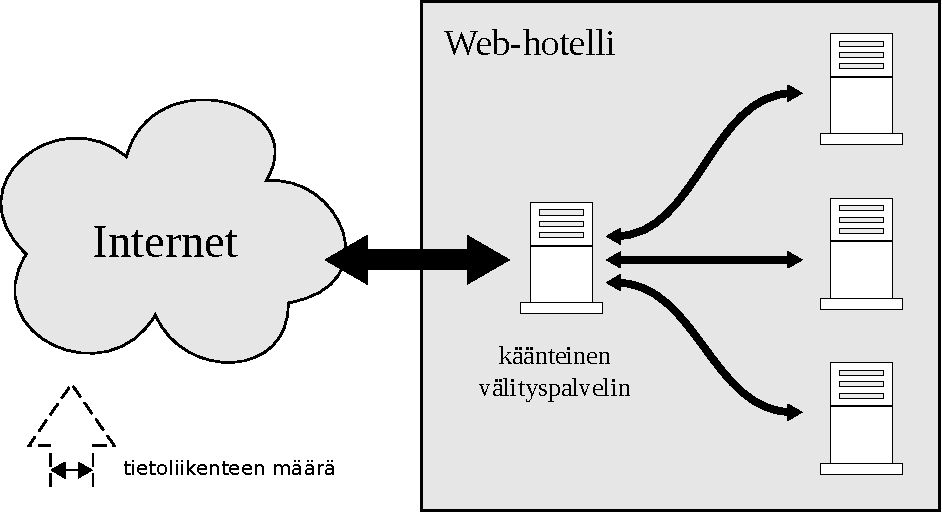
\includegraphics[width=12cm]{pics/reverseproxy.pdf}
\caption{Käänteisen välityspalvelimen toiminta.}
\label{reverseproxy}
\end{figure}

\section{Pilvivälimuisti}

Edellä kuvattu käänteinen välityspalvelin ei ole riittävä ratkaisu
kuormituksen tasaamiseen, kun kyse on laajamittaisesta
Web-palveluntarjonnasta. Käänteinen välityspalvelin vähentää
Web-palvelinten kuormitusta, mutta ei vähennä eikä hajauta palvelun
verkkoliikennettä. Jotta maailmanlaajuiset palvelut voitaisiin
toteuttaa ilman maakohtaisia erillissivustoja, tarvitaan keinoja
kuormituksen jakamiseen verkkotopologisesti edullisesti.

Eräs ratkaisu ongelmaan on sijoittaa välimuistipalvelimia
eri maantieteellisille alueille. Palvelimet säilövät välimuistiinsa harvoin
muuttuvia sivuja ja muita staattisia resursseja. Sivulle tulevat
kyselyt voidaan ohjata näille palvelimille esimerkiksi aluekohtaisten
nimipalveluiden avulla~\cite{geodns}. Kuvassa \ref{cloudcache} havainnollistetaan
järjestelmän toimintaa.

Käytännössä tällaisen järjestelmän rakentaminen ja ylläpito on
kallista, koska se vaatii toimintaa useiden valtioiden alueilla ja
lukuisien palveluntarjoajien kanssa. Ratkaisuna tähän ongelmaan on kehitetty
pilvivälimuistipalveluita.
Yksi suosituimmista näistä on Akamai Technologiesin
\textit{Web Ap\-plic\-a\-tion Accelerator}~\cite{akamai}. Järjestelmä
koostui kesäkuussa 2010 yhteensä 65~000 palvelimesta, jotka
sijaitsevat 70 eri valtion alueella. Käyttäjän tekemät kyselyt
ohjataan automaattisesti sopivimpaan Akamain palvelimeen. Sopivin
palvelin valitaan yhteyden luotettavuuden ja nopeuden
perusteella. Palvelu voi noutaa ennakolta kaiken sivulla sijaitsevan
staattisen sisällön, jolloin näiden osien välittäminen ei kuormita
varsinaisia Web-palvelimia lainkaan.

Pilvivälimuistin haittapuolena on se, että Web-palveluntarjoaja ei näe
suoraan sivustolle tulevia kyselyitä, koska monet kyselyt eivät etene
välimuistipalvelua syvemmälle. Tällöin tilastointi ja erilaisten tietomurtojen
tunnistaminen on vaikeampaa. Monet välimuistipalveluntarjoajat, Akamai
mukaanlukien, tarjoavat kuitenkin asiakkailleen monipuolisia tilastointipalveluita.

\begin{figure}[htp]
\centering
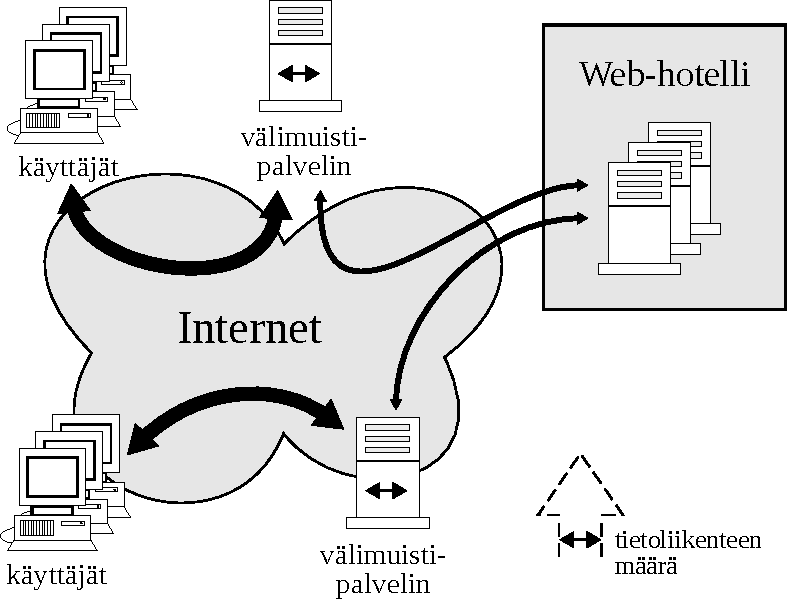
\includegraphics[width=12cm]{pics/cloudcache.pdf}
\caption{Pilvivälimuistin toiminta.}
\label{cloudcache}
\end{figure}
